\chapter{Metodología y Diseño de la Solución}\label{cap5}

\section{Metodología de desarrollo}
\label{sec:metodologia}

Para la planificación y ejecución de este Trabajo de Fin de Grado, se ha adoptado una \textbf{metodología de desarrollo iterativa e incremental}, inspirada en los principios ágiles. Esta elección se fundamenta en la naturaleza del proyecto, que combina la investigación de tecnologías emergentes (sistemas GraphRAG, agentes LLM) con la construcción de un prototipo de software funcional. A diferencia de un modelo en cascada, este enfoque se adapta a la naturaleza exploratoria del trabajo, permitiendo construir el sistema en ciclos cortos donde cada iteración produce un incremento funcional, ofreciendo ventajas clave como la flexibilidad, la gestión de la incertidumbre y la entrega de valor temprana.
La necesidad de cambios constantes a lo largo del proyecto validó esta elección: al incorporar una componente de investigación, al inicio no existía una visión completamente definida de la versión final, y los ciclos de prueba, error y aprendizaje permitieron ir modelando el sistema de forma incremental.


\newpage
\subsection{Fases del Proyecto}
El desarrollo del proyecto se estructuró en cinco fases lógicas, que se alinean con los capítulos de esta memoria y cuyo cronograma se detalla en la Tabla~\ref{tab:cronograma}. Las semanas concretas son orientativas; así, por ejemplo, la investigación se prolongó a lo largo de todo el proyecto, especialmente al término de cada iteración, con el fin de identificar mejoras sobre la base ya obtenida.

\begin{description}
    \item[Fase 1: Investigación y Definición (Semanas 1-4).] Se realizó una revisión bibliográfica exhaustiva, se definieron los objetivos del proyecto y se identificaron las tecnologías clave (Ollama, NetworkX, etc.).
    \item[Fase 2: Análisis y Diseño (Semanas 5-7).] Se formalizaron los requisitos funcionales (RF) y no funcionales (RNF), se diseñó la arquitectura general de la solución y se definieron los componentes principales del sistema.
    \item[Fase 3: Desarrollo Incremental (Semanas 8-12).] Núcleo del trabajo práctico, subdividido en tres incrementos funcionales que se detallan en el Anexo \ref{anexo:planificacion}:
        \begin{enumerate}
            \item \textbf{Incremento 1 (MVP - Núcleo RAG):} Desarrollo del pipeline de ingesta, chunking jerárquico y RAG básico para un solo documento.
            \item \textbf{Incremento 2 (Sofisticación con Grafo):} Implementación del grafo estructural y semántico, búsqueda híbrida y re-ranking.
            \item \textbf{Incremento 3 (Inteligencia de Agentes):} Integración de los agentes para optimización de consultas y selección de estrategia, y soporte para múltiples documentos.
        \end{enumerate}
    \item[Fase 4: Pruebas y Evaluación (Semanas 13-14).] Verificación del cumplimiento de los requisitos y evaluación de la calidad de las respuestas del sistema.
    \item[Fase 5: Documentación (Semanas 15-16).] Redacción final de esta memoria y preparación de la defensa.
\end{description}

\newpage
A continuación se presenta un resumen del cronograma, expresando de manera aproximada la carga de trabajo en cada una de las fases del proyecto. Si bien en la práctica el desarrollo resultó más complejo que lo recogido en la tabla, esta ofrece una síntesis representativa del mismo.
\begin{table}[H]
    \centering
    \renewcommand{\arraystretch}{1.3}
    \caption{Cronograma de Fases e Hitos Principales del Proyecto.}
    \label{tab:cronograma}
    \begin{tabularx}{\textwidth}{|l|l|X|}
    \hline
    \textbf{Fase} & \textbf{Semanas} & \textbf{Hitos y Entregables Clave} \\
    \hline
    \textbf{1. Investigación y Definición} & 1 - 4 & Objetivos definidos. Estado del arte completado. Tecnologías seleccionadas. \\
    \hline
    \textbf{2. Análisis y Diseño} & 5 - 7 & Documento de requisitos (Cap. 2). Diseño de arquitectura y componentes (Cap. 3). \\
    \hline
    \textbf{3. Desarrollo Incremental} & 8 - 12 & Código fuente de los tres incrementos funcionales completado. Ver Anexo \ref{anexo:planificacion} para el detalle de las tareas. \\
    \hline
    \textbf{4. Pruebas y Evaluación} & 13 - 14 & Plan de pruebas ejecutado. Análisis de resultados cualitativos y cuantitativos. \\
    \hline
    \textbf{5. Documentación} & 15 - 16 & Redacción y entrega de la memoria final del TFG. \\
    \hline
    \end{tabularx}
\end{table}

\newpage
\subsection{Herramientas de Apoyo a la Metodología}
Para la gestión eficaz de este proceso, se utilizaron herramientas estándar en la industria del desarrollo de software.

\subsubsection{Control de Versiones con Git}
El código fuente del proyecto se gestionó en una rama privada, dado que parte de sus contenidos podría ser confidencial para la empresa, como ocurre con algunos documentos de prueba. La rama de trabajo no puede adjuntarse públicamente; en su lugar, se ha habilitado una rama con documentos de origen público que reproduce la misma estructura. El modelo de ramificación empleado fue muy sencillo y constaba de los siguientes elementos:
\begin{itemize}
    \item \texttt{main}: Rama principal que contiene siempre la versión más estable y funcional del código. En concreto, todas las ramas se integraban una vez por incremento para verificar que las funcionalidades operasen conjuntamente de forma correcta.
    \item \texttt{feature/nombre-tarea}: Ramas de corta duración creadas para desarrollar una nueva funcionalidad o corregir un error. Una vez completada y probada, la rama se fusionaba con \texttt{main}; en la mayoría de los casos se creaba una rama por cada requisito funcional.
\end{itemize}
El uso de mensajes de commit descriptivos aseguró la trazabilidad de cada cambio realizado en el código.

\subsubsection{Gestión de Tareas con Kanban}
El seguimiento de las tareas de cada incremento se realizó mediante un tablero \textbf{Kanban} en la herramienta Trello. El tablero se estructuró en cuatro columnas principales: \textit{Backlog}, \textit{Pendiente (To Do)}, \textit{En Progreso (In Progress)} y \textit{Finalizado (Done)}. Este enfoque visual permitió priorizar el trabajo, limitar el trabajo en curso a una o dos tareas simultáneamente para mantener el foco, y tener una visión clara del progreso. En el \textbf{Anexo \ref{anexo:kanban}} se presentan capturas de pantalla del estado del tablero al finalizar cada incremento.

\subsection{Definición de Terminado (Definition of Done)}
Para asegurar la calidad y consistencia del trabajo en cada incremento, se estableció una "Definición de Terminado" (Definition of Done). Una tarea no se consideraba finalizada hasta que cumplía con todos los siguientes criterios:
\begin{itemize}
    \item El código asociado a la funcionalidad está implementado y cumple con los requisitos.
    \item El código ha sido auto-revisado y refactorizado para asegurar su legibilidad, con los comentarios correspondientes en aquellas funcionalidades que pudiesen llegar a causar confusión.
    \item Se han realizado pruebas unitarias o de integración informales para verificar que la nueva funcionalidad no introduce regresiones.
    \item El código ha sido fusionado (\textit{merged}) a la rama \texttt{main} del repositorio Git.
    \item La tarjeta correspondiente en el tablero Kanban ha sido movida a la columna \textit{Finalizado (Done)}.
\end{itemize}

Todas estas medidas, en especial el control de versiones con Git y el tablero Kanban, resultaron fundamentales para no perder tiempo identificando cuál era la siguiente tarea, además de facilitar la reversión de cambios de forma sencilla.

\newpage
\section{Arquitectura general de la solución}
\subsection{Arquitectura y Diseño del Sistema}

Para la construcción de esta solución se barajaron una serie de patrones. Finalmente, se optó por un patrón de \textbf{Arquitectura en capas}.
La elección se fundamenta en la propia necesidad de separación de las distintas responsabilidades del sistema, en específico aportando una modularidad al mismo.

Por ejemplo, al cambiar del uso de un modelo local al de una API de pago (GPT-4o-mini en las pruebas de evaluación), únicamente fue necesario modificar un único módulo, gracias a dicha modularidad.
La mantenibilidad también mejora por el mismo motivo: ante cualquier cambio, no es necesario modificar la totalidad de los módulos.
La cohesión, al tener los componentes separados, permite una comprensión más clara del sistema, sin necesidad de recorrer un único fichero de miles de líneas en busca de una funcionalidad concreta.

\subsection{Capas de la Arquitectura}

La Arquitectura de este sistema se organiza en \textbf{cuatro capas}:

\subsubsection{Capa de Presentación}

En este caso, mediante una interfaz \textbf{CLI} (también se probaron interfaces sencillas con Gradio).
Cuando se probó a implementar con GUI, esta se mantuvo en su propio documento.
Para mantenerlo sencillo con CLI, se implementa en la función \texttt{interactive\_chat()}, que es el punto de entrada desde el cual el usuario puede comunicarse con el resto de la aplicación.

\subsubsection{Capa de Lógica}

Es el corazón del sistema.
Dado que la lógica es compleja, está separada en distintos documentos. En concreto:

\paragraph{Orquestador Inteligente (\texttt{SmartDocumentProcessor}):}
Este es el componente central.
Recibe la consulta del usuario y dirige todo el flujo de la misma hasta la obtención de la respuesta.

\paragraph{Agentes:}
\begin{itemize}
    \item \textbf{Agente de Estrategia (\texttt{DocumentStrategyAgent}):}
    Es un subcomponente llamado por el orquestador.
    Su tarea es, a partir de la \textit{query} realizada por el usuario, decidir si utilizar partes del documento (empleando GraphRAG) o si, por el contrario, la pregunta requiere necesariamente de un contexto completo, como puede ser un resumen del mismo.

    \item \textbf{Agente de Optimización de Consulta (\texttt{DocumentStrategyAgent}):}
    Subcomponente llamado por el orquestador cuya tarea es refinar la consulta del usuario.
    Se explicará con más detalle en su respectivo punto, pero resumidamente formula una pregunta más apta para la búsqueda con GraphRAG, en caso de que el Agente de Estrategia haya decidido esa ruta.
\end{itemize}

\paragraph{Núcleo GraphRAG (\texttt{PDFRAGSystemWithNetworkX}):}
Es el principal motor de la búsqueda, análisis del grafo, generación del contexto que se dará al LLM y creación de la respuesta generada para el usuario.

\subsubsection{Capa de Datos}

En este caso, al no trabajar con documentos recurrentes, no se mantiene persistencia de los \textit{embeddings} fuera de la ejecución.
(Es una de las propuestas futuras que depende exclusivamente de las necesidades del usuario).

Por tanto, al momento de la entrega, la capa de datos es únicamente el sistema de ficheros en el que se almacena el grupo de documentos con el que alimentar al LLM a la hora de proporcionarle contexto.

\subsubsection{Servicios Externos}

Dependiendo de las necesidades de la implementación concreta:

\begin{itemize}
    \item \textbf{LLM Local:}
    Utiliza un servicio como \textit{Ollama}, que escucha peticiones HTTP y es capaz de devolver respuestas generadas localmente.
    Al recibir una petición, el servicio ejecuta el modelo en la máquina del usuario, procesa la entrada y devuelve la respuesta correspondiente.

    \item \textbf{API Externa:}
    Se emplea un cliente de API externa para conectarse a otro proveedor (por ejemplo, GPT u otro).
    Es más sencillo de desplegar y evita los problemas de albergar un servidor localmente, aunque conlleva un coste en función del uso.
\end{itemize}

\subsection{Conclusión}

Esta estructura permite que cada uno de los componentes se centre en una tarea específica y, por tanto, lograr la \textbf{modularidad} establecida en el RNF-01, además del resto de ventajas anteriormente mencionadas.


\section{Casos de uso}

\newpage
\subsection{CU-01 Subida de Documentos}
\begin{table}[H]
\centering
\renewcommand{\arraystretch}{1.3} % más espacio entre filas
\begin{tabularx}{\textwidth}{|l|X|}
\hline
\textbf{Identificador} & CU-01 \\
\hline
\textbf{Nombre} & Subida de Documentos \\
\hline
\textbf{Objetivo} & Determinar si el documento que proporciona el usuario es de un tipo válido. \\
\hline
\textbf{Actores} & Principal: Usuario \\
\hline
\textbf{Precondiciones} & Debe de tenerse uno o varios archivos en formato texto. \\
\hline
\textbf{Disparador (Trigger)} & Introducir el documento o bien en la carpeta destinada, o al ejecutarlo en GUI en el TextBox. \\
\hline
\textbf{Flujo principal} &
1. Introducción del documento. \newline
2. Éxito. \newline
3. Error, documento no válido. \\
\hline
\textbf{Flujos alternativos} & No. \\
\hline
\textbf{Excepciones} & E1: Error de características (Tamaño...). \newline E2: Error de Formato (Intentar introducir un .zip, .mp4...). \\
\hline
\textbf{Postcondiciones} & El sistema obtiene los documentos. \\
\hline
\textbf{Entradas} & Documentos (Sin limite aparente de los mismos), en formatos aceptados por los extractores de texto, .pdf, .docx... , y con un tamaño total inferior a 500mb. \\
\hline
\textbf{Salidas} & Documentos con formato comprobado. \\
\hline
\textbf{Prioridad / Frecuencia} & Alta. \\
\hline
\end{tabularx}
\caption{Ficha del caso de uso CU-01.}
\label{tab:CU-01}
\end{table}

\begin{figure}[H]
    \centering
    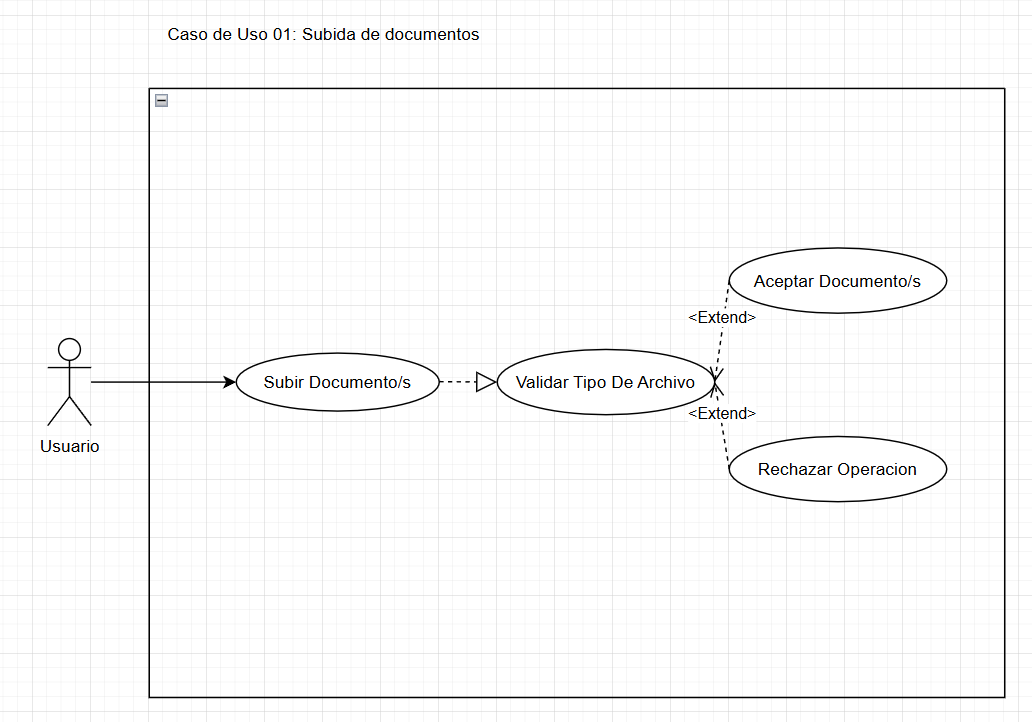
\includegraphics[width=0.75\linewidth]{images/CU-01.png}
    \caption{CU-01}
    \label{fig:CU-01}
\end{figure}

\paragraph{Explicación conceptual:}
Al subir un documento, el sistema debe validar que el tipo de archivo sea compatible: no se aceptan documentos de audio (como archivos MP4) ni imágenes (jpg, png, etc.). Los PDF con texto no seleccionable (equivalentes a imágenes) son aceptados técnicamente, pero no se garantiza el éxito del procesamiento; la aplicación de OCR fue considerada y se realizaron pruebas preliminares, aunque se trata de una mejora futura, ya que su uso limitaría la calidad del \textit{chunking} dinámico.
Este es un control básico de entrada; en esta misma fase se realizan además el resto de comprobaciones necesarias (tamaño, etc.).

\subsection {CU-02 Preprocesamiento Y Segmentación}

\begin{table}[H]
\centering
\renewcommand{\arraystretch}{1.3} % más espacio entre filas
\begin{tabularx}{\textwidth}{|l|X|}
\hline
\textbf{Identificador} & CU-02 \\
\hline
\textbf{Nombre} & Preprocesamiento Y Segmentación \\
\hline
\textbf{Objetivo} & Obtener únicamente información relevante en el texto, hacer una separación óptima y crear embeddings. \\
\hline
\textbf{Actores} & Principal: Chunk Extractor \newline Secundarios: Ninguno \\
\hline
\textbf{Precondiciones} & Debe haberse ejecutado el CU-01, y depende del flujo, el CU-03 (Se entra en detalle en la explicación), pues para el procesado hacen falta documentos. \\
\hline
\textbf{Disparador (Trigger)} & CU-01 \\
\hline
\textbf{Flujo principal} &
1. CU-01 Correcto. \newline
2. Procesamiento de documentos Indexables. \newline
3. Obtención de embeddings. \\
\hline
\textbf{Flujos alternativos} & Procesamiento de documentos no indexables (OCR) (Futuro). \newline Obtención de embeddings. \\
\hline
\textbf{Excepciones} & Los errores de este caso deberían haber sido prevenidos en el CU-01. \\
\hline
\textbf{Postcondiciones} & Al finalizar este CU obtenemos los embeddings con los que trabajaremos. \\
\hline
\textbf{Entradas} & Los documentos que recibe del CU-01. \\
\hline
\textbf{Salidas} & En este caso concreto, los embeddings no se almacenan de manera persistente, por lo que no se mantienen post-ejecución. \\
\hline
\textbf{Prioridad / Frecuencia} & Alta. \\
\hline
\textbf{Dependencias} & CU-01. \\
\hline
\end{tabularx}
\caption{Ficha del caso de uso CU-02.}
\label{tab:CU-02}
\end{table}

\begin{figure}[H]
    \centering
    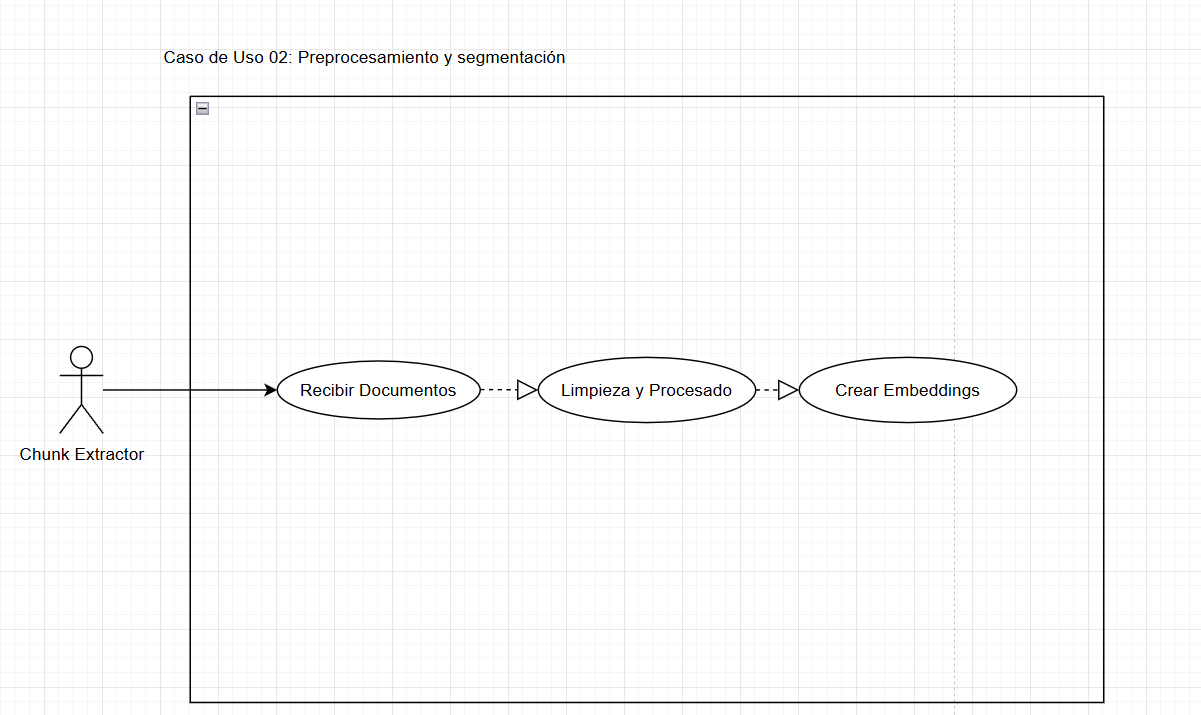
\includegraphics[width=0.75\linewidth]{images/CU-02.png}
    \caption{CU-02}
    \label{fig:CU-02}
\end{figure}

\paragraph{Explicación conceptual:}
Al recibir el documento, el sistema realiza la limpieza y el preprocesado necesarios para su posterior transformación en \textit{embeddings}. Si bien actualmente los \textit{embeddings} no se emplean como mecanismo de persistencia, representan una mejora futura clave al integrar bases de datos vectoriales.

La lógica de extracción se implementa en el módulo (\texttt{chunk\_extractor.py}), orientado a preservar la estructura jerárquica del documento —aspecto fundamental para GraphRAG— mediante los siguientes procesos:

\begin{enumerate}
    \item \textbf{Intento de extracción de hipervínculos:}

    Esta función (\texttt{extract\_links\_with\_detailed\_debug(pdf\_path)}) se encarga de:
    \begin{itemize}
        \item \textbf{Identificar enlaces internos:} Utiliza la librería \texttt{PyMuPDF} para detectar anotaciones de tipo \textit{link} que apunten a páginas dentro del mismo documento.
        \item \textbf{Filtrado por márgenes:} Mediante la función \texttt{get\_page\_margins}, ignora cualquier enlace fuera del área central (10\% de margen), descartando encabezados y pies de página.
        \item \textbf{Recuperación de respaldo (Fallback):} Si el PDF no posee hipervínculos activos, aplica una búsqueda mediante expresiones regulares (\texttt{index\_pattern}) en las primeras 6 páginas para detectar un índice textual basado en numeración y puntos suspensivos.
    \end{itemize}

    \item \textbf{Organización jerárquica del índice:}

    Esta función (\texttt{organizar\_indice(hyperlinks\_data)}) es crítica para la posterior construcción del grafo en NetworkX. Se encarga de:
    \begin{itemize}
        \item \textbf{Detección de niveles:} Analiza la estructura numérica (ej. ``1.2.1'') mediante \texttt{extract\_\allowbreak number\_struc\-ture} para determinar la profundidad de cada sección.
        \item \textbf{Inferencia por indentación:} En ausencia de numeración clara, utiliza la coordenada horizontal ($X$) del enlace para identificar subsecciones (una mayor $X$ implica un nivel de jerarquía inferior).
        \item \textbf{Asignación de parentesco:} Establece relaciones ``Padre-Hijo'' comparando los prefijos numéricos o retrocediendo en la lista de elementos para encontrar el ancestro común más cercano.
    \end{itemize}

    \item \textbf{Extracción estricta de texto entre secciones:}
    Esta función (\texttt{extract\_text\_be\-tween\_sec\-tions\_strict(pdf\_path, links\_data)}) se encarga de:
    \begin{itemize}
        \item \textbf{Localización visual:} No se limita a copiar el texto de la página; utiliza \texttt{find\_title\_\allowbreak in\_page} con algoritmos de lógica difusa (\textit{fuzzy matching}) y comprobación de estilo (negritas) para hallar el punto exacto donde comienza y termina cada sección.
        \item \textbf{Segmentación precisa:} Define el \textit{chunk} desde el final del título de la sección actual hasta el inicio del título de la siguiente sección, permitiendo que un mismo apartado abarque múltiples páginas.
        \item \textbf{Normalización:} Excluye metadatos irrelevantes y limpia el ruido visual del texto extraído.
    \end{itemize}

    \item \textbf{Persistencia de segmentos:}

    Esta función (\texttt{save\_chunks\_to\_file(chunks, output\_file)}) se encarga de:
    \begin{itemize}
        \item \textbf{Serialización:} Almacena los fragmentos procesados en un archivo de salida, incluyendo metadatos clave: ID de sección, título normalizado, nivel jerárquico y referencia al padre.
        \item \textbf{Formateo:} Estructura el contenido de forma legible para facilitar la depuración de las fases posteriores del \textit{pipeline} de RAG.
    \end{itemize}
\end{enumerate}

\subsection {CU-03 Análisis de la pregunta y decisión del agente}

\begin{table}[H]
\centering
\renewcommand{\arraystretch}{1.3} % más espacio entre filas
\begin{tabularx}{\textwidth}{|l|X|}
\hline
\textbf{Identificador} & CU-03 \\
\hline
\textbf{Nombre} & Análisis de la pregunta y decisión del agente. \\
\hline
\textbf{Objetivo} & Según la pregunta, decidir si se utilizan fragmentos parciales del documento (\textit{chunks}) y optimizar la consulta para una recuperación mediante GraphRAG más precisa. \\
\hline
\textbf{Actores} & Principal: Usuario \newline Secundarios: Agente de decisión. \\
\hline
\textbf{Precondiciones} & Deben haberse completado el CU-01 y el CU-02 para disponer de los \textit{embeddings}. \\
\hline
\textbf{Disparador (Trigger)} & Fin del CU-02. \\
\hline
\textbf{Flujo principal} &
1. El usuario hace una pregunta. \newline
2. El agente la recibe. \newline
3. Se decide si se responde con documentos completos o con las secciones de contenido. \newline
4. Si es por secciones el Agente proporciona una pregunta Optimizada para la búsqueda. \\
\hline
\textbf{Flujos alternativos} & En caso de ser el documento completo no se ejecuta el caso 4 del flujo principal. \\
\hline
\textbf{Excepciones} & Los errores posibles deberían haber sido manejados en CU-01. \\
\hline
\textbf{Postcondiciones} & Al finalizar se dispone de la decisión sobre el tipo de respuesta y, en caso de seleccionarse la ruta por secciones, de la consulta optimizada. \\
\hline
\textbf{Entradas} & Pregunta. \\
\hline
\textbf{Salidas} & Tipo de respuesta, pregunta optimizada. \\
\hline
\textbf{Prioridad / Frecuencia} & Alta. \\
\hline
\textbf{Dependencias} & Incluye: CU-01, CU-02. \\
\hline
\end{tabularx}
\caption{Ficha del caso de uso CU-03.}
\label{tab:CU-03}
\end{table}

\begin{figure}[H]
    \centering
    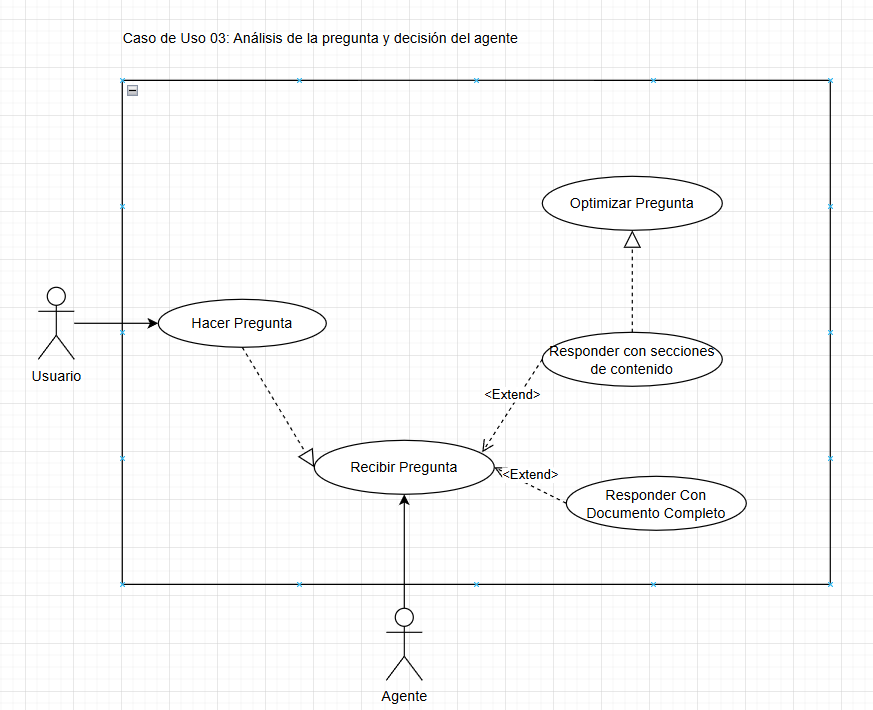
\includegraphics[width=0.75\linewidth]{images/CU-03.png}
    \caption{CU-03}
    \label{fig:CU-03}
\end{figure}

\paragraph{Lógica del Agente de Selección de Estrategia:}
Para optimizar el consumo de recursos y la precisión de las respuestas, se ha implementado un agente inteligente (\texttt{DocumentStrategyAgent}) que actúa como capa intermedia entre la consulta del usuario y el motor de recuperación. Su función principal es determinar si la consulta requiere una búsqueda local (RAG) o una comprensión global del documento.

Este proceso, integrado en la clase \texttt{SmartDocumentProcessor}, sigue la siguiente lógica:

\begin{enumerate}
    \item \textbf{Análisis Dinámico de la Consulta:}
    La función (\texttt{analyze\_query}) envía la pregunta del usuario junto con metadatos del documento (número de páginas, tipo de archivo) a un modelo de lenguaje (LLM). El agente evalúa dos escenarios:
    \begin{itemize}
        \item \textbf{Acceso Parcial (RAG):} Se activa si la consulta busca datos específicos, hechos puntuales o secciones concretas (ej. ``¿Cuál es el presupuesto en la sección 3?'').
        \item \textbf{Acceso Total (Full Document):} Se activa si la consulta requiere entender el documento como un todo, realizar resúmenes globales o encontrar inconsistencias transversales.
    \end{itemize}

    \item \textbf{Clasificación y Razonamiento:}
    El agente no solo devuelve una decisión, sino que mediante la función (\texttt{\_parse\_decision}) extrae:
    \begin{itemize}
        \item \textbf{Estrategia:} \textit{Partial} o \textit{Full}.
        \item \textbf{Nivel de Confianza:} Un valor numérico que permite auditar la fiabilidad de la elección.
        \item \textbf{Razonamiento:} Una explicación textual de por qué se eligió dicha ruta, mejorando la interpretabilidad del sistema.
    \end{itemize}

    \item \textbf{Ejecución de Rutas de Respuesta:}
    Dependiendo de la decisión y del modo de operación seleccionado, el procesador (\texttt{process\_query}) ejecuta:
    \begin{itemize}
        \item \textbf{Modo RAG Individual/Consolidado:} Utiliza el sistema de grafos (\texttt{NetworkX}) para recuperar subsecciones relevantes de uno o varios documentos.
        \item \textbf{Modo de Contexto Extendido:} En caso de elegir la estrategia \textit{Full}, se invoca la función \texttt{\_process\_full\_documents}, que reconstruye el documento manteniendo el orden jerárquico de secciones y lo inyecta en una ventana de contexto ampliada (hasta 60.000 tokens).
    \end{itemize}

    \item \textbf{Interfaz Interactiva y Control de Flujo:}
    A través de (\texttt{interactive\_chat}), el sistema permite al usuario alternar entre modos de respuesta (Individual vs. Consolidada) y activar la visualización de los grafos generados, permitiendo una depuración en tiempo real del proceso de recuperación.
\end{enumerate}

\subsection {CU-04 Generación de Respuesta}

\begin{table}[H]
\centering
\renewcommand{\arraystretch}{1.3} % más espacio entre filas
\begin{tabularx}{\textwidth}{|l|X|}
\hline
\textbf{Identificador} & CU-04 \\
\hline
\textbf{Nombre} & Generación de Respuesta \\
\hline
\textbf{Objetivo} & Secuencia de Generación de la Respuesta. \\
\hline
\textbf{Actores} & Principal: Usuario \newline Secundarios: LLM \\
\hline
\textbf{Precondiciones} & Debemos haber completado el CU-03. \\
\hline
\textbf{Disparador (Trigger)} & Fin del CU-03. \\
\hline
\textbf{Flujo principal} &
1. El usuario selecciona el tipo de respuesta. \newline
2. Se ejecuta el proceso según la respuesta. \newline
3. El modelo Genera la respuesta. \\
\hline
\textbf{Flujos alternativos} & 1-Eran necesarios los documentos completos y exceden la ventana de contexto del modelo en uso. \newline 2-Se cortará el excedente. \\
\hline
\textbf{Excepciones} & Si se corta el excedente la respuesta puede ser poco indicativa de la realidad. \\
\hline
\textbf{Postcondiciones} & El usuario recibe la respuesta según formato solicitado. \\
\hline
\textbf{Entradas} & Lo obtenido en los otros CU. \\
\hline
\textbf{Salidas} & Respuesta en formato texto. \\
\hline
\textbf{Prioridad / Frecuencia} & Alta. \\
\hline
\textbf{Dependencias} & Incluye: CU-01, CU-02, CU-03. \\
\hline
\end{tabularx}
\caption{Ficha del caso de uso CU-04.}
\label{tab:CU-04}
\end{table}

\begin{figure}[H]
    \centering
    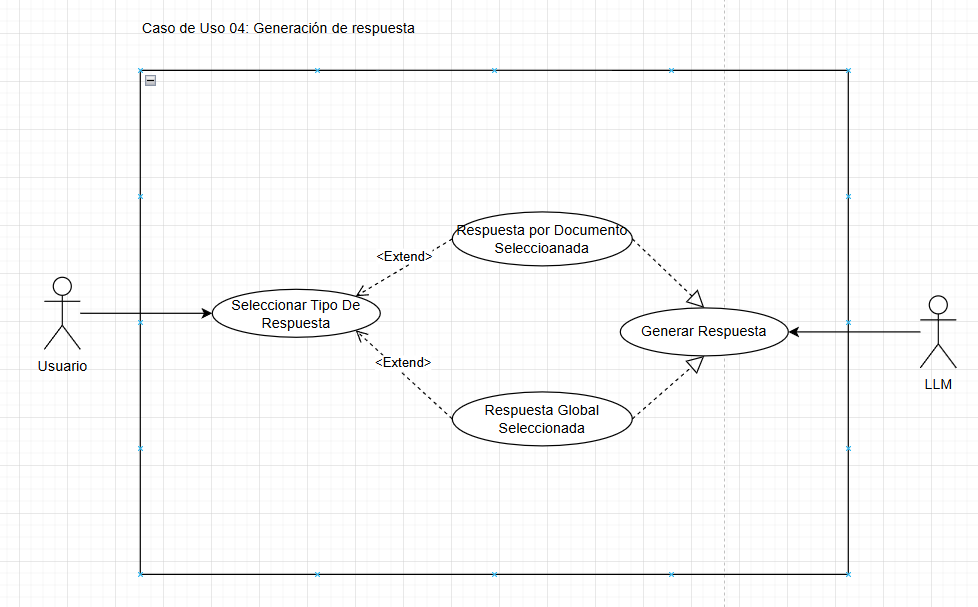
\includegraphics[width=0.75\linewidth]{images/CU-04.png}
    \caption{CU-04}
    \label{fig:CU-04}
\end{figure}
\newpage

\paragraph{Casos de Uso e Interacción (CU-04):}
La lógica de interacción se centraliza en el método \texttt{inter\-active\_chat}, el cual materializa el caso de uso \textbf{CU-04: Seleccionar Tipo de Respuesta}. Como se observa en el diagrama de la Figura 5.4, el usuario interactúa con el sistema para decidir cómo se procesará la información recuperada por el LLM.

Este componente gestiona la ejecución mediante los siguientes estados y opciones:

\begin{enumerate}
    \item \textbf{Modo 1: Respuestas Individuales (Default):}
    Corresponde a la extensión \textit{<<Extend>> Respuesta por Documento Seleccionada}. El sistema genera una respuesta independiente por cada archivo PDF cargado, utilizando grafos de conocimiento locales. Es ideal para comparar normativas o pliegos técnicos de distintos proveedores de forma aislada.

    \item \textbf{Modo 2: Respuesta Consolidada:}
    Activa la extensión \textit{<<Extend>> Respuesta Global Seleccionada}. Mediante la función \texttt{generate\_consolidated\_graph\_response}, el sistema realiza un análisis transversal de todos los documentos, unificando los grafos de NetworkX para ofrecer una visión de conjunto.

    \item \textbf{Gestión de Observabilidad (Visualización):}
    El sistema permite activar la visualización de grafos en tiempo real (\texttt{visualize\_graphs = True}). Esta funcionalidad genera representaciones gráficas (PNG) de las relaciones de conocimiento detectadas, lo que permite al usuario (o desarrollador) validar la calidad de la recuperación semántica.

    \item \textbf{Ciclo de Control:}
    La implementación utiliza un bucle persistente que permite cambiar la estrategia de consulta (\texttt{modo 1/2}) y las opciones de depuración sin necesidad de reiniciar el sistema ni volver a procesar los documentos, optimizando así el tiempo de respuesta en sesiones de análisis extensas.
\end{enumerate}

El flujo finaliza con la intervención del actor \textbf{LLM}, que recibe el contexto estructurado según el modo seleccionado para generar la respuesta final al usuario.

\newpage
\section{Diagramas de comportamiento}
\begin{figure}[htb!]
    \centering
    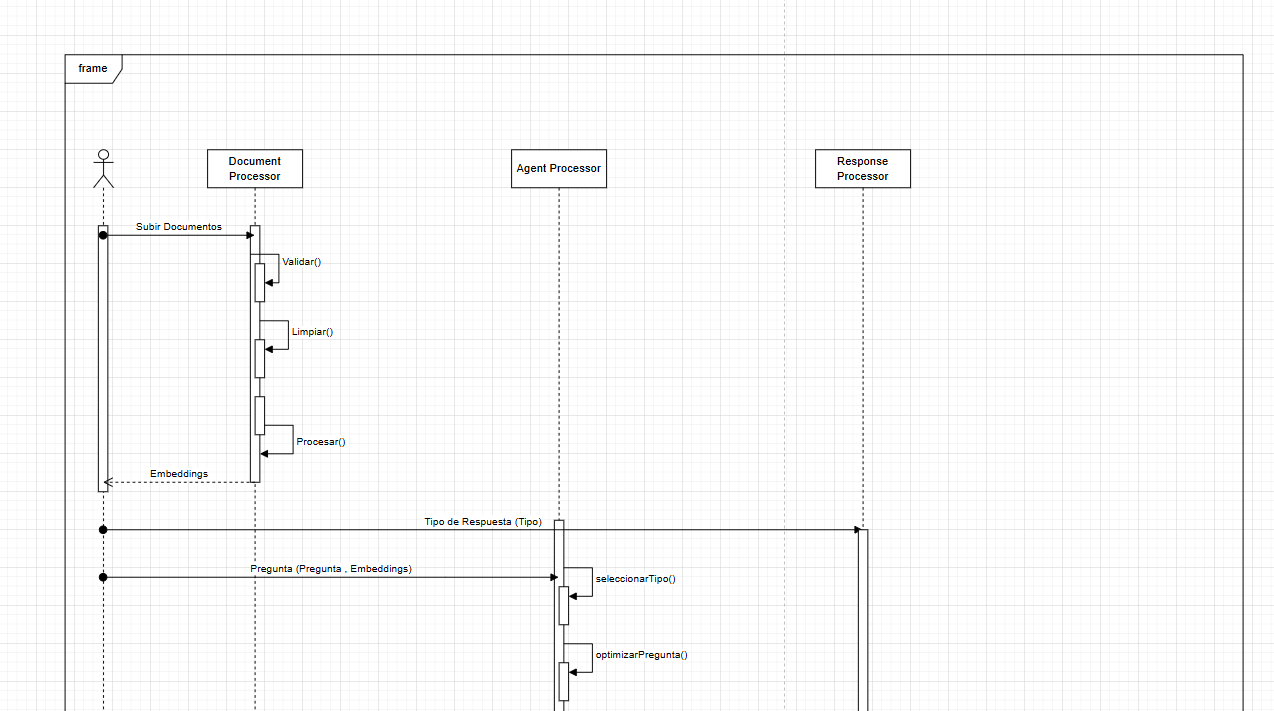
\includegraphics[width=1\linewidth]{images/Seq-01.png}
    \label{fig:seq01}
\end{figure}

\begin{figure}[htb!]
    \centering
    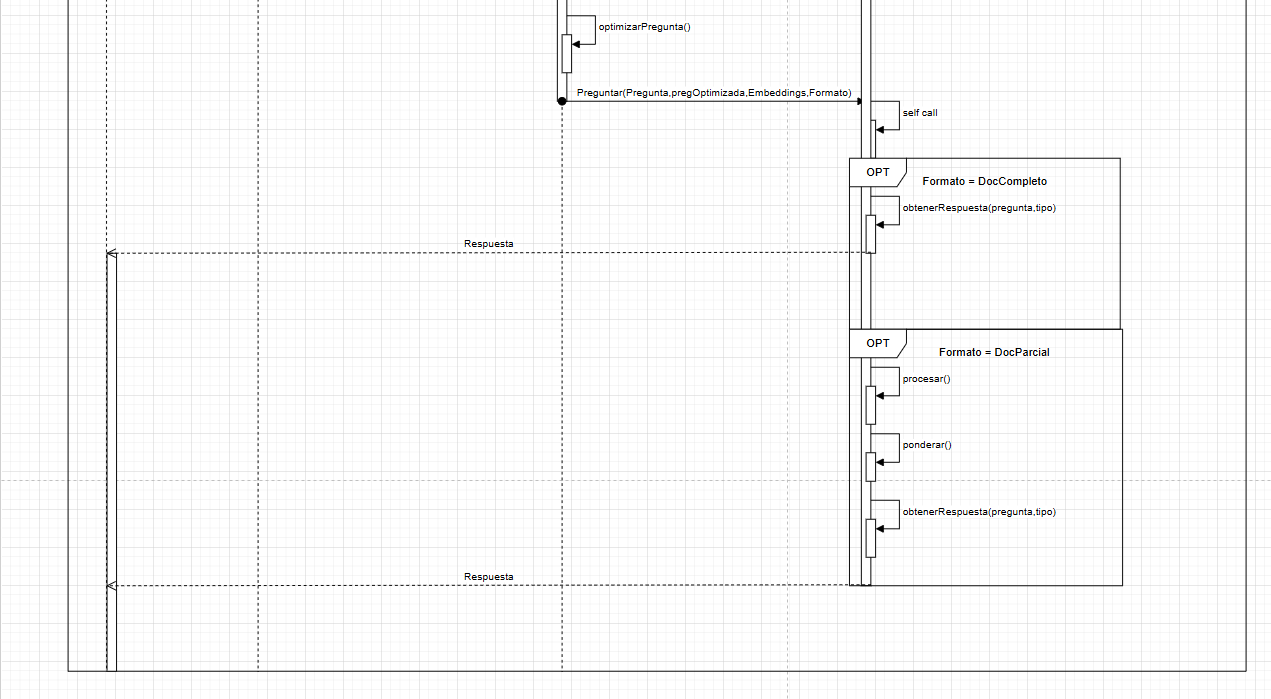
\includegraphics[width=1\linewidth]{images/Seq-02.png}
    \caption{Diagrama de Secuencia}
    \label{fig:seq02}
\end{figure}

\newpage

\paragraph{Pipeline de Procesamiento y Resolución de Consultas:}
En este diagrama de secuencia se muestra cómo sería el flujo (uno de los posibles) dentro del sistema.
El comportamiento dinámico del sistema se articula a través de una arquitectura de pipeline dividida en tres fases fundamentales, coordinando la preparación de la base de conocimiento con la ejecución de agentes inteligentes para la generación de respuestas.

\begin{enumerate}
    \item \textbf{Fase de Ingestión y Estructuración (\textit{Document Processor}):}
    En esta etapa, el sistema transforma documentos PDF no estructurados en una red de conocimiento jerárquica:
    \begin{itemize}
        \item \textbf{Validación y Normalización:} Se realiza una limpieza profunda del texto para eliminar ruido visual y asegurar la integridad de los datos procesados.
        \item \textbf{Segmentación Jerárquica:} Utilizando la lógica de \texttt{chunk\_extractor.py}, el sistema identifica secciones y subsecciones, preservando las relaciones de dependencia originales del documento.
        \item \textbf{Indexación Vectorial:} Se generan \textit{embeddings} para cada segmento, permitiendo búsquedas semánticas eficientes en fases posteriores.
    \end{itemize}

    \item \textbf{Fase de Orquestación y Decisión (\textit{Agent Processor}):}
    Una vez consolidada la base de datos, el sistema actúa como un agente inteligente de decisión:
    \begin{itemize}
        \item \textbf{Análisis de Intención:} El \texttt{DocumentStrategyAgent} evalúa la consulta para determinar si se requiere una búsqueda de datos específicos (RAG) o un análisis global (Contexto Completo).
        \item \textbf{Optimización Semántica:} En la ruta RAG, se ejecuta un proceso de refinamiento de la consulta para extraer términos clave, maximizando la precisión de la recuperación en el grafo.
    \end{itemize}

    \item \textbf{Fase de Recuperación y Generación (\textit{Response Processor}):}
    La fase final integra la información recuperada con el modelo de lenguaje:
    \begin{itemize}
        \item \textbf{Recuperación sobre Grafo (\textit{GraphRAG}):} El sistema no solo busca fragmentos aislados, sino que utiliza \texttt{NetworkX} para realizar una ``Propagación Familiar''. Esto permite incluir secciones ascendentes (padres) y descendentes (hijos) del nodo relevante, con el objetivo de proporcionar al LLM un contexto estructural más completo que el fragmento aislado.
        \item \textbf{Ponderación Híbrida:} Se combinan métricas de similitud de coseno, BM25 y centralidad de grafo (\textit{PageRank}) para seleccionar los fragmentos más informativos.
        \item \textbf{Generación de Respuesta:} El LLM procesa el contexto curado para ofrecer una respuesta que respete la jerarquía del documento, citando explícitamente las secciones de origen.
    \end{itemize}
\end{enumerate}

\begin{figure}
    \centering
    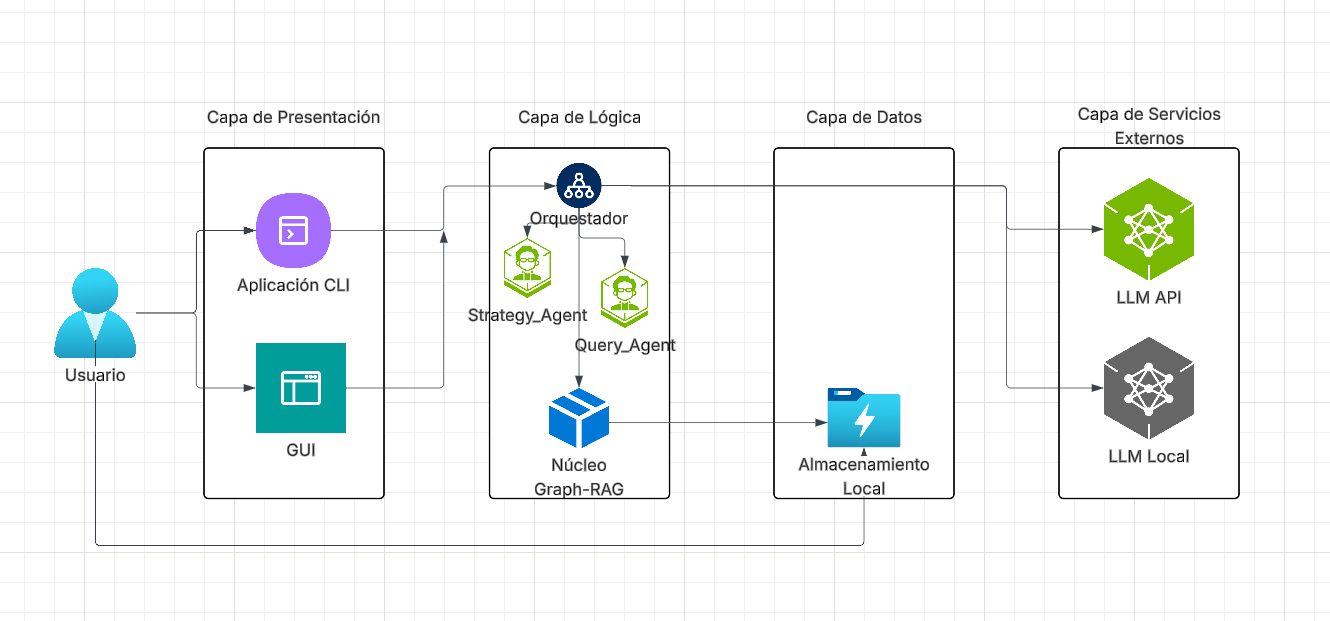
\includegraphics[width=1\linewidth]{images/Diagrama_Arquitectura.png}
    \caption{Diagrama de Arquitectura}
    \label{fig:Arquiteture_Diagram}
\end{figure}

\begin{figure}
    \centering
    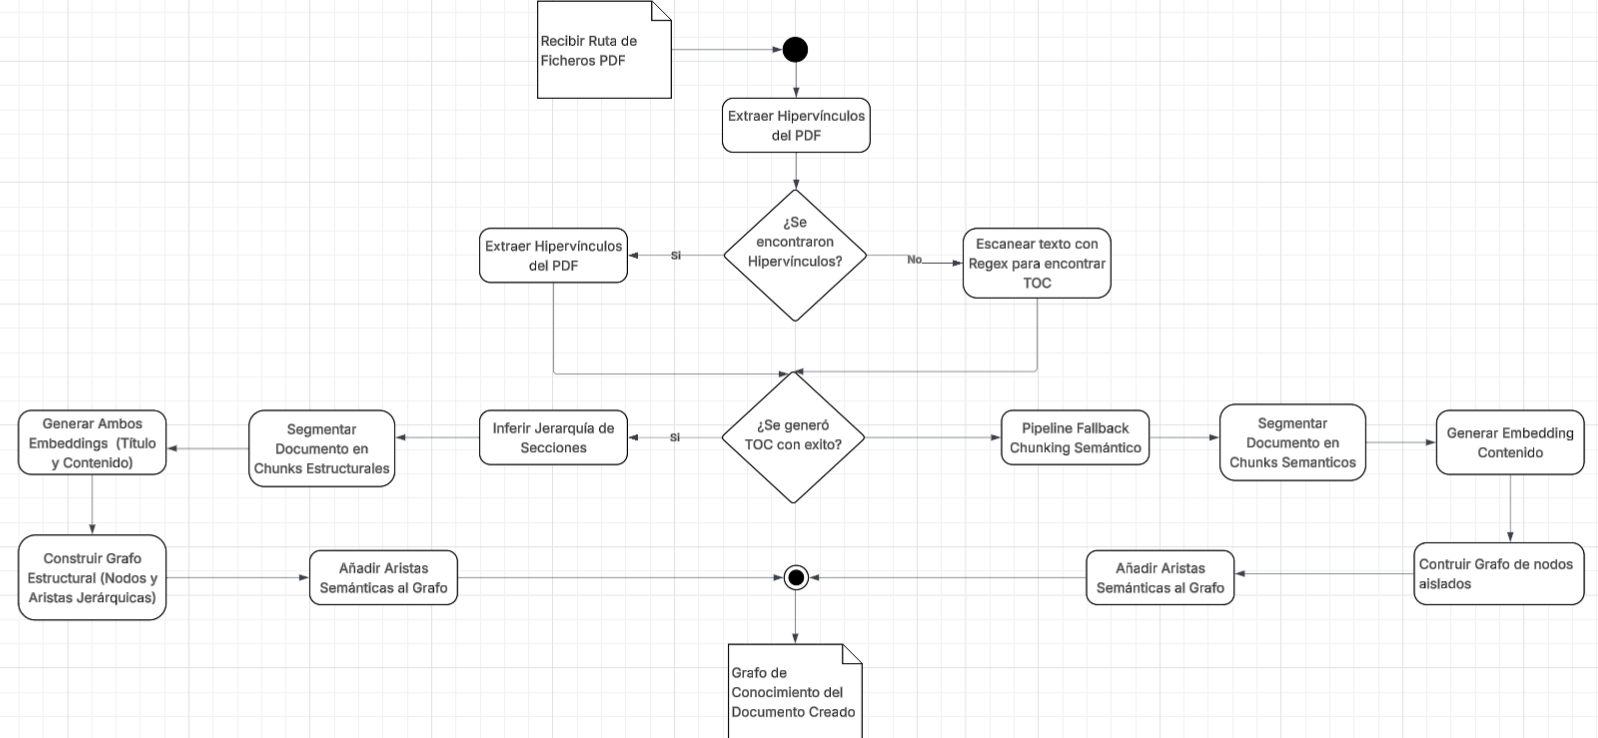
\includegraphics[width=1\linewidth]{images/Diagrama_Actividad_CU-02.png}
    \caption{Especificación diagrama de Actividad CU-02}
    \label{fig:activitydiag01}
\end{figure}
